\chapter{Trigger Logic and Data Taking}
\label{sec:trigger}
The trigger is a logic circuit that will be able to select muons
that do not cross the setup and stop in one of the planes.
In this way we can measure the decay time of the muon by using the
trigger signal generated by a stopping muon as 
a start signal of the
time measurement.
If we take \autoref{fig:Setup} as reference of the experimental apparatus we start by
connecting each PMTs of plane 0 like \autoref{fig:logig_plane0}.
We need an AND gate for each half-plane, because we want a signal from both PMTs.
This way we reduce the background noise.
Meanwhile the OR gate is needed since there are two half-planes
and a muon can cross either two.\\
\begin{figure}[h]
\begin{center}
\includegraphics[width=80 mm,scale=0.5]{figures/Cattura2.png}
\end{center}
\caption{Logic circuit of plane 0.}
\label{fig:logig_plane0}
\end{figure}
We repeat the process for plane 1. For plane 2
we want a NOT gate at the end of the OR gate, so that we have a signal when no muons cross P2
to make sure that the muon has actually stopped. The P0, P1 and NOT P2 will be connect to an AND
gate so that only when all of them generate a signal we can have the trigger signal as
shown in \autoref{fig:trigger_system}.

\begin{figure}[h]
\begin{center}
\includegraphics[width=100mm]{figures/Cattura3.png}
\end{center}
\caption{Trigger system.}
\label{fig:trigger_system}
\end{figure}

For the time measurement we use a couple of TDCs in series since we need a least 10$\;\symup{\mu}$s
and the max time measurable for this TDC is 5$\;\symup{\mu}$s.
The TDC is controlled by a crate controller that sends the commands and gets the information
from the module, while a DAQ code (LabVIEW) communicates with the crate controller
in this way:
\begin{enumerate}
  \item When a start signal arrives at the TDC the 8 clocks start running
  \item If 1 of the clocks of the TDC has a stop before the time limit (5$\;\symup{\mu}$s) then a memory location called LAM is set to 1
  \item The crate controller reads the memory location of the LAM continuously. If it is set to 
   1, the crate stops reading the LAM, reads the measurement and then clears them to start again.
\end{enumerate}
If there is no stopping signal in the 5$\;\symup{\mu}$s time limit the LAM will never be set
to 1 so the crate controller will never stop the measurement and clear the memory leading to a 
DAQ problem. We can solve this by taking a copy of the start signal, delay
it by 4.7$\;\symup{\mu}$s and connect it to one of the clocks of the TDC. This way we have
a fake stop that will set the LAM to 1 to prevent the problem.
With this in mind we build the circuit shown in \autoref{fig:daq}.\\
\begin{figure}[h]
\begin{center}
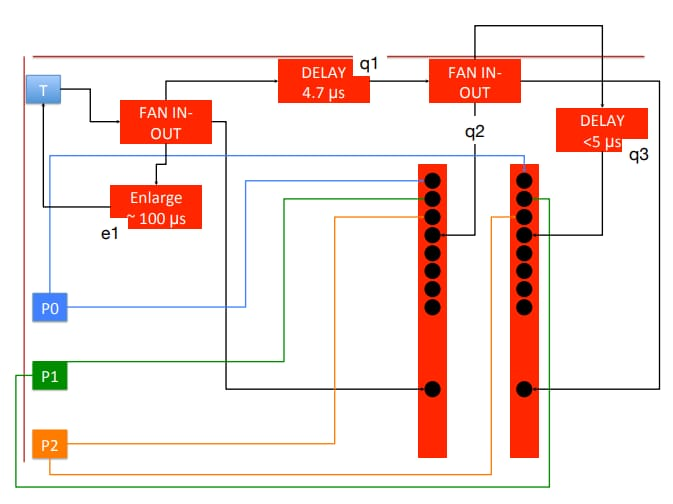
\includegraphics[width=100mm]{figures/cattura4.png}
\end{center}
\caption{Data aquistion circuit.}
\label{fig:daq}
\end{figure}

The first three clocks will be connected to the P0, P1 and P2 in search for an electron
appearance signal. The start for the first TDC is given by the trigger from which we take a copy
of and delay it by 4.7$\;\symup{\mu}$s (q1). From this we take 3 copies with a fan-in-fan-out:
\begin{enumerate}
\item the first will be used as the fake stop for the first TDC (q2),
\item the second will be the start of the second TDC,
\item the third will be delayed again by a time $<5\;\symup{\mu}$s and used as a fake stop for the second TDC (q3).
\end{enumerate}
The last thing is to make sure that no trigger is generated in the deadtime of the DAQ
so we take the signal,s enlarge it up to 100$\;\symup{\mu}$s and send back to the logic
unit that provides the trigger in the VETO input (e1).\\